% Report skeleton for DD2430 Group 3: Agentic AI Compiler (Ericsson).
% Target: 6-10 pages, IEEE two-column conference format.
% Each section lists what belongs there and a rough page budget.
% Delete the guidance comments and \todo notes as the text gets written.

\documentclass[conference]{IEEEtran}

\usepackage[utf8]{inputenc}
\usepackage[T1]{fontenc}
\usepackage{amsmath}
\usepackage{graphicx}
\usepackage{float}
\usepackage{booktabs}
\usepackage{xcolor}
\usepackage{listings}
\usepackage{hyperref}
\usepackage{tikz}
\usetikzlibrary{arrows.meta, positioning}

\newcommand{\todo}[1]{\textcolor{red}{[TODO: #1]}}

\lstset{basicstyle=\footnotesize\ttfamily, breaklines=true, frame=single}

\begin{document}

\title{An Agentic Optimization Loop Around the XLA Compiler:\\
Algorithmic Rewrites of JAX Programs with Language Models}

\author{
\IEEEauthorblockN{Joel Maharena, John Christensen, Lidya Nasser, Sara Strandberg}
\IEEEauthorblockA{DD2430, KTH Royal Institute of Technology\\
Project in collaboration with Ericsson}
}

\maketitle

\begin{abstract}
% 150-200 words, written last: problem, approach, main quantitative result, main limitation.
Compilers such as XLA fuse and schedule operations but cannot redesign an
algorithm, so such rewrites still depend on human experts. We build an
agentic optimization loop around JAX and XLA in which a language model reads
the lowered program and its profile, proposes a source-level rewrite, and
receives correctness and latency feedback from an evaluator that rejects
incorrect candidates before timing them. We evaluate on one NVIDIA L4 GPU
against vanilla XLA, using 13 single-rewrite programs, three longer programs
with planted inefficiencies, and five realistic kernels. Measurement noise
is about $\pm3\%$, so only speedups above $1.03\times$ count. A single model
call found the expert rewrite for all 13 simple programs, but produced a
correct result on only 2 of 9 runs of the planted programs, where multi-call
search often matched or exceeded the expert. On realistic code, three of
five kernels showed no gain over XLA. On the two kernels with causal
attention, a tool-using agent reached $1.8$--$3.2\times$ and
$1.13$--$1.54\times$ by skipping the blocks of scores above the causal
diagonal, a rewrite found independently by two model families. The main limitation is
scope: one GPU, five realistic kernels, and one to three runs per
configuration.
\end{abstract}

\begin{IEEEkeywords}
compilers, XLA, JAX, large language models, agents, performance optimization
\end{IEEEkeywords}

% ---------------------------------------------------------------------------
\section{Introduction}
% About 1 page.
% - Running AI models is costly, so speeding up inference saves money.
% - Lowering pipeline: experts redesign algorithms, engineers write kernels,
%   compilers fuse and schedule automatically. Compilers use fixed rewrite rules.
% - Idea: an LLM agent that reads compiler output and profiles, rewrites code,
%   and measures the result, like a human performance engineer.
% - Scope: inference (forward pass) on one NVIDIA L4 GPU.
% - Contributions as a short bulleted list.

Training and serving large AI models are among the major costs in today's AI industry. Improving training and inference efficiency can therefore directly be translated into significant financial savings. There are several approaches to achieve this, but optimization today often involves a combination of manual and automated processes. Engineers manually redesign algorithms using mathematical and hardware-aware tricks, such as FlashAttention \cite{dao2022flashattention}, or write and tune device-specific kernels using programming frameworks such as CUDA, Triton and Pallas. At a lower level, compilers such as XLA automatically optimize computation graphs through techniques such as operator fusion, scheduling and lowering operations to target accelerators. However, compilers are generally limited to predefined optimization rules. They can fuse and schedule operations, but they cannot typically redesign an algorithm or find alternative ways of performing a computation, as in the case of FlashAttention. 

Redesigning algorithms and tuning device kernels still depends largely on human expertise and can be a time-consuming process. A language model can read a lowered program, form a hypothesis about why it is slow, and suggest a new version of the code and thus in this project we build an agentic AI system that supplements a compiler to make AI models faster by automating the algorithmic design optimization. Given a program in JAX, the agent repeatedly tries to rewrite the code into a faster version while preserving correctness. It stops when it reaches its attempt budget, or when the model itself replies that it has nothing further to try. 
\newline

Our contributions are:
\begin{itemize}
  \item {An agent loop around JAX/XLA that observes the lowered program and its profile, proposes a rewrite, checks correctness, and measures latency.
}
  \item {An evaluator that rejects incorrect candidates before any timing is done, together with a noise-floor check so small timing differences are not counted as real speedups.}

  \item {An evaluation on an NVIDIA L4 against vanilla XLA (the original JAX program compiled with no agent rewrite), on 13 short programs with one known inefficiency each, 3 longer programs with planted inefficiencies, and five realistic JAX workloads with no planted inefficiency. On the first two sets we also compare to hand-written expert rewrites.}
\end{itemize}

% ---------------------------------------------------------------------------
\section{Related Work}
% About 0.75 page. Compare each line of work to ours.
\subsection{Hand-designed algorithmic rewrites}
FlashAttention by Dao et al. \cite{dao2022flashattention} is a good example of manual algorithmic design optimization that brought significant speedups. Standard attention requires materialising the intermediate attention matrix $QK^T$in GPU memory before applying softmax. For long sequences, this matrix becomes large and requires substantial memory access. Data needs to be moved between the GPU's fast on-chip memory (SRAM) and high-bandwidth memory (HBM), and repeatedly reading and writing intermediate results causes slowdowns. FlashAttention addresses this by restructuring the attention computation using tiling, where the inputs are divided into smaller blocks that fit in the GPU's fast on-chip memory (SRAM). This reduces the need to repeatedly read and write intermediate results to high-bandwidth memory (HBM), while preserving the exact attention computation. The authors demonstrated significant speedups, including a 3x speedup on GPT-2 compared to standard attention. This demonstrates how redesigning an algorithm around hardware characteristics can achieve performance improvements beyond simply optimising the execution of the original operations.

\subsection{Machine-learning compilers}
JAX \cite{jax} is a Python library that is designed for high performance numerical computing and machine learning models. It gives Numpy like interface to computations that run on CPU, GPU or TPU and has built in Just in Time (JIT) compilation via OpenXLA \cite{openxla}. XLA is an open source compiler designed for high performance computing and machine learning models through intermediate representations such as StableHLO and by optimizing computations graphs at lower level such as operation fusion, for example if a sequence of elementwise operations can be fused into a single kernel.


JAX and the XLA compiler are effective at optimising the computations that have been written. However, they cannot change the algorithm itself. For instance, multiplying by a diagonal matrix is still treated as a matrix product unless the programmer has already written it using broadcasting. Similarly, a chain of matrix products may be evaluated in the order it appears, even when a different association would reduce the amount of work. These are the kinds of limitations that our agent tries to address by finding equivalent but more optimised computations. The agent rewrites the JAX program that is fed into it and then lets XLA compile the new version. The lowered program and runtime profile are used as feedback about what the compiler did and did not manage to optimize on its own.


\subsection{LLM agents for kernel and code optimization}
Research by Ouyang et al. \cite{ouyang2025kernelbench} uses language models to write and improve GPU kernels directly. KernelBench frames the task as writing a fast GPU kernel from a reference implementation and evaluates whether the generated kernels are correct and faster than the baseline. Another related work by Lange et al. from Sakana AI \cite{lange2025robust} emphasises the importance of verification and careful benchmarking, since an agent evaluated only on speed may exploit weaknesses in the evaluation process and produce results that are not correct.

In our case, the agent does not write device kernels. Instead, it rewrites JAX code, and XLA still compiles the result, so the agent and the compiler work together rather than replacing each other. Additionally, the feedback given to the agent is not only a pass/fail score and a latency number. It also includes compiler output, such as StableHLO, and timing profiles, which the agent can use to form a hypothesis about where time is spent. Our goal is an algorithmic rewrite of a whole program, rather than writing a device kernel.

% ---------------------------------------------------------------------------
\section{Problem Description}
% About 0.5 page. Make the task precise enough that the results can be judged.
% - Input: a pure JAX function f and example inputs x.
% - Output: a function g with g(x) close to f(x) within tolerance, and lower latency.
% - Correctness: |g(x) - f(x)| <= atol + rtol * |f(x)|, with the values used.
% - Objective: median latency on the target device, excluding compilation.
% - Baseline: vanilla XLA compilation of f.
Let \(f\) be a JAX function that returns a single finite floating-point array, and let \(x\) be a tuple of array inputs with the shapes and dtypes that \(f\) expects. The agent should produce a new function \(g\) such that

\[g(x) \approx f(x)\]

within the tolerance, for every element,

\[|g(x)-f(x)| \leq atol + rtol|f(x)|\]

and

\[t_{\text{median}}(g) < t_{\text{median}}(f)\]

Here, \(t_{\text{median}}\) is the median execution time of the compiled program on the target device, measured over repeated calls after compilation and warm-up. Compilation time and the first call are therefore excluded.

The tolerances are chosen per program. By default, we use a relative tolerance of \(10^{-5}\) and an absolute tolerance of \(10^{-6}\). The planted programs and the softmax use a relative tolerance of \(10^{-4}\). For programs mainly consisting of matrix products, we use a looser relative tolerance of \(10^{-2}\), since float32 operations on GPUs may use reduced precision. On a separate test input \(x'\) with the same shapes, \(g\) must also produce results within the required tolerance on that input. This helps ensure that the rewritten function works beyond just the original input values.

We measure performance using the speedup relative to the original program compiled with vanilla XLA:

\[\text{speedup}(g) =\frac{t_{\text{median}}(f)}
{t_{\text{median}}(g)}.
\]

Since the agent may try several rewrites, the three fastest correct candidates are timed again on a third input \(x''\), and we report the best of these (Section~\ref{sec:evaluation}).


% ---------------------------------------------------------------------------
\section{Methodology and Implementation}
% About 2 pages. One subsection per component, plus a system diagram.
\subsection{System overview}
The system wraps a language model around the existing JAX/XLA tool chain
and leaves the compiler itself unchanged. Its input is a \emph{task}: a
reference JAX function $f$, the source text of $f$ that the model may read,
the tolerances $(\mathit{rtol}, \mathit{atol})$, and three input cases with
the same shapes and dtypes, generated from fixed seeds: $x$, $x'$ and $x''$.
The model only ever runs code on $x$. The held-out case $x'$ is used only to
check correctness, and $x''$ only for the final re-measurement.

Every attempt has the same four steps (Fig.~\ref{fig:system}).
\emph{Observe}: the reference, and later the candidates, are compiled, and
their compiled form and latency are summarized as text. \emph{Propose}: the
model replies with a JSON object that contains Python source defining a
function \texttt{candidate}. \emph{Verify}: the evaluator compiles the
candidate and checks it against the reference on $x$ and $x'$.
\emph{Measure}: a correct candidate is timed against the reference. The
speedup, or the reason the candidate was rejected, is added to what the
model sees next. When the budget is used up, the best candidates are timed
again on $x''$, and that number is the result.

The loop has two drivers. In the \emph{fixed loop}, every model call
produces one candidate. The single-call, best-of-$n$ and chain methods in
Section~\ref{sec:evaluation} use it. In the \emph{tool agent}, the model
chooses its next action itself. Both drivers share the compiler interface,
the evaluator and the final re-measurement, but they are two complete search
strategies: the tool agent also gets a different summary of the compiled
program, can time parts of the program, and can send up to four candidates
in one turn.

\begin{figure}[!t]
  \centering
  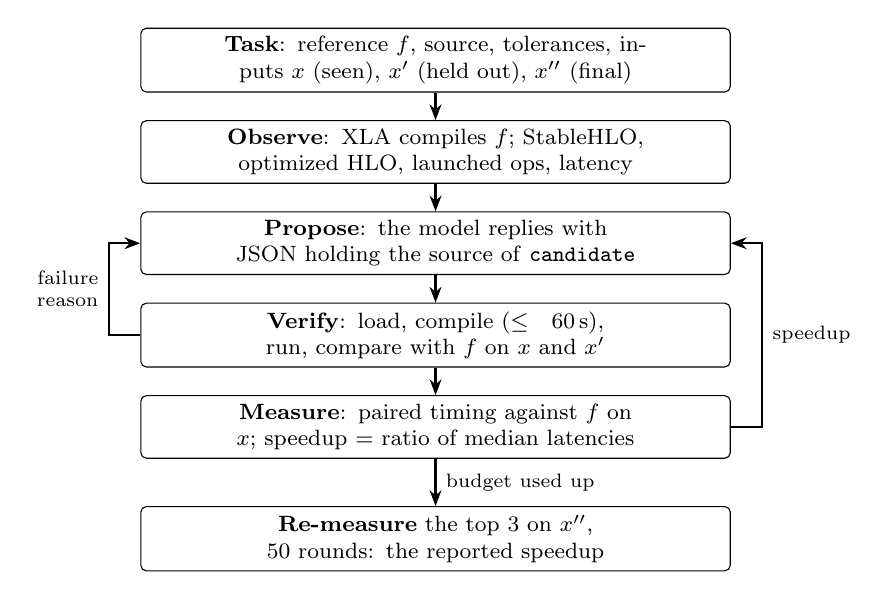
\begin{tikzpicture}[
      node distance=3.5mm,
      box/.style={draw, rounded corners=2pt, align=center, font=\footnotesize,
                  text width=0.60\columnwidth, inner sep=3pt},
      side/.style={align=left, font=\scriptsize},
      flow/.style={-{Stealth[length=2mm]}, thick}]
    \node[box] (task) {\textbf{Task}: reference $f$, source, tolerances, inputs $x$ (seen), $x'$ (held out), $x''$ (final)};
    \node[box, below=of task] (observe) {\textbf{Observe}: XLA compiles $f$; StableHLO, optimized HLO, launched ops, latency};
    \node[box, below=of observe] (propose) {\textbf{Propose}: the model replies with JSON holding the source of \texttt{candidate}};
    \node[box, below=of propose] (verify) {\textbf{Verify}: load, compile ($\le 60$\,s), run, compare with $f$ on $x$ and $x'$};
    \node[box, below=of verify] (measure) {\textbf{Measure}: paired timing against $f$ on $x$; speedup = ratio of median latencies};
    \node[box, below=6mm of measure] (final) {\textbf{Re-measure} the top 3 on $x''$, 50 rounds: the reported speedup};
    \draw[flow] (task) -- (observe);
    \draw[flow] (observe) -- (propose);
    \draw[flow] (propose) -- (verify);
    \draw[flow] (verify) -- (measure);
    \draw[flow] (measure) -- node[right, side] {budget used up} (final);
    \draw[flow] (measure.east) -- ++(4mm,0) |- node[pos=0.25, right, side]
      {speedup}
      (propose.east);
    \draw[flow] (verify.west) -- ++(-4mm,0) |- node[pos=0.25, left, side, align=right]
      {failure\\ reason} (propose.west);
  \end{tikzpicture}
  \caption{The optimization loop around the XLA compiler. The compiler is not
  modified; the model only rewrites the JAX source that XLA compiles. In the
  tool agent the model can also ask for the observe step, or for timings of
  parts of the program, before it proposes a candidate.}
  \label{fig:system}
\end{figure}

\subsection{Compiler interface}
All compilation goes through one function, \texttt{compile\_program}$(f, x)$.
It traces $f$ with \texttt{jax.jit} for the shapes and dtypes of $x$, lowers
it to StableHLO, and lets XLA compile it for the device. It returns the
executable and two texts: the StableHLO before XLA's optimization passes,
and the optimized HLO after them. The optimized HLO shows which operations
XLA actually launches, for example whether a product with a diagonal matrix
was compiled into a full matrix product.

On the L4, XLA's autotuner can take very long. For one short program
(pairwise distances of 1024 points) it compiled for more than 15 minutes,
and a compilation cannot be stopped once it has started. One such candidate
would therefore stall a whole run. Before a candidate is compiled, it is
exported with \texttt{jax.export} and compiled in a separate child process.
That process is killed after 60\,s, and the candidate is then rejected. A
program that finishes in time is compiled again in the main process, so
every checked program is compiled twice.

\subsection{Profiler}
The profiler times one program on its own. It moves the inputs to the
device, compiles the program, and records the compile time. It then makes
one warm-up call followed by 20 timed calls, and waits for each call with
\texttt{block\_until\_ready}. JAX launches GPU work asynchronously, so
without the wait only the launch would be timed. The profiler reports the
median time of the calls. It does not break the time down by kernel.

The full optimized HLO is too long for a prompt. For the transformer block it
runs to tens of thousands of characters, most of them the bodies of fused
computations and source locations. The fixed loop shows the beginning
of the StableHLO and of the optimized HLO. The tool agent gets a
summary instead, with four parts:
\begin{itemize}
  \item the operations XLA launches, from the entry computation and the loop
    and branch bodies it calls, counted by opcode, with the fusion kind or
    the library call (for example a cuBLAS matrix product);
  \item XLA's own estimates of FLOPs and bytes accessed;
  \item the floating-point types that occur in the compiled program;
  \item the beginning of the launched computations, with metadata
    removed.
\end{itemize}
For a candidate, the operation counts are also given as changes against the
reference, such as \mbox{\texttt{dot 3 -> 1}}. The floating-point types are also
stored with each candidate. They show a change of type, such as to bfloat16,
but not a float32 matrix product computed in reduced precision, so we also
searched the source of every winning candidate for precision arguments.

\subsection{Evaluator}
The evaluator compares a candidate $g$ with the reference $f$. It returns
either both latencies, or the stage at which $g$ failed and a message. The
stages come in this order:
\begin{enumerate}
  \item \emph{load}: the reply could not be parsed, or its source does not
    define a function \texttt{candidate};
  \item \emph{compile}: tracing or compilation failed or exceeded 60\,s;
  \item \emph{execute}: the compiled program raised an error when run;
  \item \emph{correctness}: the output on $x$ or on $x'$ does not match;
  \item \emph{benchmark}: the candidate failed while it was being timed.
\end{enumerate}
An output matches when it has the reference's shape and dtype, both outputs
contain only finite values, and every element satisfies
$|g(x)-f(x)| \le \mathit{atol} + \mathit{rtol}\,|f(x)|$. When an output does
not match, the message gives the largest error as a multiple of the allowed
error, the share of elements outside the tolerance, and the worst element.
This tells the model whether a candidate is nearly right, with a rounding or
summation-order problem at about $1\times$ the allowed error, or computes
something else, at $10^4\times$. A candidate is timed only after it has
passed on both inputs, so a fast but wrong program never gets a speedup.

Timing reuses the two executables that the main process compiled for the
correctness check, and each is first called once without timing. In each of
$n$ rounds, each program is then called once, and the program that goes
first alternates between rounds. In early tests we timed one program
completely before the other, and two identical programs then measured 1\%
to 3\% apart. Each latency is the median over the rounds ($n = 20$ during
the search), and the speedup is the ratio of the two medians. Compilation
time is not included, and peak memory is not measured.

\emph{Final re-measurement.} Picking the fastest of many noisy measurements overstates the winner. A
candidate that was simply lucky in its timing can come out on top. When a
run ends, whichever method produced it, the three fastest correct candidates
are therefore evaluated again on the fresh input $x''$, with 50 timing
rounds. The reported speedup is the best of these re-measured values.

\subsection{LLM policy and prompting}
The \emph{policy} decides what the model is asked and what is done with its reply. We use two policies, a fixed loop and a tool agent, and three model providers.

\paragraph{Fixed loop}
In the fixed loop, each model call produces one candidate. The prompt
contains the device, the input shapes, the reference's median latency, the
truncated StableHLO and optimized HLO, and the reference source. After the
first attempt, the prompt also lists every earlier attempt with its source,
its rationale and its outcome. The outcome is either the speedup and both
latencies, or the failure stage and the message.
The prompt then names the best attempt so far, shows its optimized HLO, and
tells the model to improve on it and not to repeat a rejected attempt.

The model replies with a JSON object
\texttt{\{"stop", "rationale", "candidate\_source"\}}. The source is run with
\texttt{exec} in a namespace that holds only \texttt{jax} and \texttt{jnp},
and must define a function named \texttt{candidate}. A reply that cannot be
used is recorded as a failed attempt at the load stage, with the reason, and
the loop continues. On this loop we build three methods. \emph{Single} is
one call. \emph{Best of $n$} is $n$ independent single calls, none of which
sees the others. \emph{Chain} is $n$ calls in one loop, so each call sees the
earlier attempts.

We used two system prompts. Our first prompt described tools such as
\emph{inspect\_compilation} that the fixed loop does not let the model call,
and let the model stop at any time. In GPU runs, \texttt{gpt-6-luna} then
sometimes answered \emph{stop} because it could not use those tools. The
\emph{original chain} in Section~\ref{sec:evaluation} uses this prompt. The
other fixed-loop methods use a second prompt, which describes what the
model actually gets and says that it cannot run anything itself. It states
the goal and where speedups can come from: XLA already fuses operations and
picks kernels, but it does not change the algorithm. The prompt also gives
rules for the code: use only JAX; keep float32 arithmetic; compute the same
function rather than an approximation that passes only because the tolerance
is loose, such as the tanh form of an exact GELU; and keep the function pure.
The model may stop only if it is sure that no rewrite can be faster.

\paragraph{Tool agent}
In the tool agent, the model sends one action per turn. The harness runs the
action and appends the result, an \emph{observation}, to a transcript. The
whole transcript is sent again on every turn. The opening message gives the
task, the device, the input dtypes and shapes, the tolerances, the reference
source, the reference's latency, the summary of its compiled form, and the
budget. There are four actions:
\begin{itemize}
  \item \emph{inspect} returns the compiled summary of the reference, of an
    earlier candidate, or of new code, compared with the reference;
  \item \emph{time} runs any function of the inputs, for example one part of
    the reference, with paired timing against the whole reference and no
    correctness check, and reports its share of the reference's time;
  \item \emph{evaluate} sends one to four candidates, each with a one-line
    idea, through the full evaluator;
  \item \emph{finish} ends the run with a summary of what was found.
\end{itemize}
\emph{Time} acts as a profiler for parts of the program. The model can see
where the time goes before it spends evaluations, which matters on long
programs with several slow parts. Every observation ends with a leaderboard
of the three fastest correct candidates, the source of the best one, and the
budget left.

A run stops when the model finishes, after 12 turns, after 16 candidate
evaluations, or after four evaluate turns in a row bring no improvement. With
12 turns, the tool agent has the same number of calls as the other methods.
Because timing is noisy, a candidate counts as an improvement only when it
beats the best so far by 5\%, which is above the noise band in
Section~\ref{sec:evaluation}. The search starts from the reference at
$1.00\times$. We first planned to stop after two evaluate turns without
improvement, but in a pilot run the model sent one candidate per turn and the
run stopped after 2 of its 12 turns, so the limit was raised to four. The
system prompt shares the goal and the code rules with the second fixed-loop
prompt. It also tells the model to inspect and time parts of a large program
before rewriting it, to try several different ideas in the first evaluate
turn, and to measure the main parts of its best candidate before finishing.

\paragraph{Language models}
All models are reached through one text interface: a call sends a system
prompt and a message and gets text back. The interface keeps no state, so
the caller sends the whole conversation each time. Gemini is called through
Google's API, and a failed request is retried. Claude models are called
through the Claude Code command-line tool in print mode, with all of its
tools turned off. OpenAI models are called through the Codex command-line
tool, in a read-only sandbox, with a medium reasoning effort.
Both command-line tools run in an empty temporary folder without the user's
settings, so they cannot read our repository. In every case the model only
returns text. Every candidate is compiled, checked and timed by our
evaluator.


\subsection{Numerical precision on the GPU}
By default XLA computes float32 matrix products on the L4 in a reduced
precision (TF32). Against a float64 result its median relative error was
$2.9\times10^{-4}$, compared with $2.4\times10^{-7}$ when JAX is told to use
the \texttt{highest} precision. Which setting applies changes both the
reference's latency and the error a rewrite may introduce, so it must be the
same for reference and candidate.

The single-rewrite suite and the planted programs run with \texttt{highest}
everywhere. Their relative tolerances are tight ($10^{-5}$ and $10^{-4}$),
and in our tests at the default precision, correct programs failed checks
this tight. The realistic kernels with matrix products have a tolerance of
$10^{-2}$, which reduced precision passes; with their
references at \texttt{highest}, a candidate could gain speed by asking for
reduced precision alone (Section~\ref{sec:kernels}). Their final runs
therefore leave the references at XLA's default precision, and we check every
winning candidate for code that changes the precision.

% ---------------------------------------------------------------------------
\section{Experimental Evaluation}
\label{sec:evaluation}
% Replacement prose for Section V. Keep the existing section labels, tables,
% listing, and cross-references in the current manuscript.
\subsection{Setup}

We ran the experiments on one NVIDIA L4 GPU on a Google Cloud
\texttt{g2-standard-4} instance, using JAX 0.12.0.1 and CUDA 12.
For the planted programs and realistic kernels, we used commit
\texttt{6a612ed}. We increased the timeout for Claude from 120 to 900
seconds so that longer replies could finish. The run records and the
script for summarizing these results are in
\texttt{results/2026-11-14-gpu}.

We tested each candidate on two inputs. The agent could see the first
input, while the second was held out for the correctness check. We
rejected candidates that took more than 60 seconds to compile or failed
either check. For candidates that passed, we alternated between timing
the reference and the candidate. We calculated speedup by dividing the
reference's median execution time by the candidate's median execution
time. Both measurements excluded compilation.

During search, we used 20 timing rounds. For the planted programs and
realistic kernels, we then took up to three of the fastest correct
candidates from each run and timed them again for 50 rounds on a fresh
input, $x''$. We report the best of these final measurements. The
single-rewrite suite was run earlier with the fixed loop and 20 timing
rounds, without this final measurement.

We used Gemini 3.6 Flash through its API, \texttt{gpt-6-luna} and
\texttt{gpt-6.1-sol} through the Codex command-line tool, and Claude
Fable 5.2 through the Claude Code command-line tool. We count one
request to a model as one call.

\subsection{Benchmarks}

The three benchmark sets address different questions. The
\emph{single-rewrite suite} tests whether the agent can improve a
program with one known inefficiency. Each of the 13 programs has an
expert rewrite for comparison. For example, one program computes a
whole matrix product even though it only needs the trace.

The \emph{planted programs} test how the search methods perform when a
program has several inefficiencies. We used causal self-attention, an
embedding layer followed by a transform, and windowed standardization.
Each contains two or three planted inefficiencies. Fixing any one of
them gave at most a $6.1\times$ speedup. Fixing all of them gave
$5.6\times$, $85\times$, and $75\times$ for the three programs,
respectively. These clean versions served as the expert rewrites for comparison.

For the \emph{realistic kernels}, we wanted to see whether the agent
could improve code with no deliberately planted inefficiency. We used a
matrix product, softmax, a fused linear layer with GELU and layer
normalization, causal attention, and a transformer block. The attention
input had two sequences, 16 heads, and 2048 tokens per sequence. We used
a relative tolerance of $10^{-2}$ for the kernels with matrix products
and $10^{-4}$ for softmax. We excluded a small GPT workload because its
reference took more than 300 seconds to compile.

\subsection{Measurement noise}

We first measured how much timing could vary when the two programs were
identical. We compared each of two MLP programs with a copy of itself
90 times. The 5th to 95th percentile range was $0.992$--$1.016\times$
for one program and $0.972$--$1.025\times$ for the other. We therefore
counted a measured speedup above $1.03\times$ as a gain. This cutoff is
based on two controls timed in pairs. Measurements from separate runs
can vary more. During search, the tool agent used a separate 5\% threshold
to decide whether a new candidate improved on the best speedup so far.
Four consecutive evaluation turns without such an improvement ended the run.

\subsection{Single-rewrite suite}
\label{sec:suite}

Table~\ref{tab:suite} compares the expert rewrites with candidates
generated by Gemini 3.6 Flash. For each of the 13 programs, the best
correct candidate from two or three attempts achieved at least 96\% of
the expert rewrite's measured speedup. We timed the expert rewrites and
agent candidates in separate runs, each against its own measurement of
the original program. Small differences between their reported speedups
can therefore reflect variation between runs. One candidate failed the
numerical correctness check and received no timing score.

\subsection{Planted programs: comparing search methods}

We ran each method three times on each of the three planted programs
using \texttt{gpt-6-luna}. The single-call method proposed one candidate.
Best of $n$ made 12 independent calls and kept the fastest correct
candidate. The chain also had 12 calls, but each call received the
earlier attempts and their results. We included the original version of
the chain, whose prompt allowed it to stop early. The tool agent chose
when to inspect, time, or evaluate code and when to finish, with a limit
of 12 calls.

Table~\ref{tab:planted} gives the results for all nine runs per method. A single call
produced a correct rewrite in two of nine runs. Best of
$n$ produced a gain above $1.03\times$ in all nine runs. The chain and
tool agent each produced a gain in eight runs, and the original chain
did so in six. On each program, every multi-call method had at least one
run that reached 85\% of the expert speedup or better. Results also
varied between runs of the same method. With three runs per program,
these counts give limited evidence about which method would perform
best on a new program.

The tool agent typically used two to five calls, although one run used
eleven. Its median run time was 132 seconds, compared with 548 seconds
for best of $n$. Best of $n$ thus gave the most consistent gains in
these experiments, while the tool agent usually needed fewer calls and
had a shorter median run time.

Feedback sometimes reinforced an earlier mistake. In one chain run,
the model misread the reference and continued from that interpretation
for seven attempts. The run ended at $1.00\times$. The original chain
stopped without a correct candidate in three runs, and the tool agent
did so once. We repeated two tool-agent runs after Codex returned an
empty reply, which the runner treated as an unavailable model. The
reported results use the repeated runs with the same code and settings.

\subsection{Realistic kernels}

The first runs exposed a problem with the precision settings. The
references used the highest matrix multiplication precision, while the
$10^{-2}$ tolerance also accepted results computed using TF32. Table~\ref{tab:precision} shows two
winning candidates that explicitly asked for reduced precision.
\texttt{gpt-6-luna} achieved $2.06\times$ on the matrix product, and
\texttt{gpt-6.1-sol} achieved $2.34\times$ on the fused layer. Both
passed the output checks without changing the algorithm.

For the final runs, we used XLA's default matrix multiplication
precision for the references. With this setting, the
\texttt{gpt-6.1-sol} tool agent measured $1.00\times$ on both the
matrix product and the fused layer, and $1.01\times$ on softmax. All
three fell below our cutoff. The single-call method produced either a
slower candidate or one that failed the correctness check on these
kernels. None of the winning candidates in the final runs explicitly
set a precision argument in its source.

Both model families found a gain on causal attention by skipping blocks
of scores above the causal diagonal. The reference computes scores for
all query--key pairs and then applies the mask. The rewrite divides the
queries into blocks. For each block it computes scores only for keys up
to the last query in that block. It still applies the mask inside the
block so that each query can attend only to its own position and
earlier positions. XLA did not produce this rewrite for the original
program in our configuration. The same change improved the attention
part of the transformer block.

Listing~\ref{lst:attention} shows the fastest attention candidate, generated by
\texttt{gpt-6.1-sol}. On the fresh input $x''$, it took 3.00~ms,
compared with 9.72~ms for the reference, a $3.24\times$ speedup. It
processed four heads at a time and split the 2048 queries into four
blocks of 512. The four query blocks needed one, two, three, and four
key blocks respectively. This computes 10 of the 16 possible score
blocks (62.5\%). The rewrite also used smaller temporary score arrays.
We did not measure how much each change contributed to the speedup.

Table~\ref{tab:kernels} shows that the tool agent achieved $1.81$--$3.24\times$ on causal
attention and $1.13$--$1.54\times$ on the transformer block. On
attention, the tool agent measured a higher speedup than the single
call in all six paired runs. On the transformer block,
\texttt{gpt-6.1-sol} produced no correct single-call candidate in three
runs. The tool agent improved on the reference in all four
transformer-block runs across the two model families.


% ---------------------------------------------------------------------------
\section{Summary and Discussion}
% About 1 page.
% - What worked, what did not, and why.
% - Limitations: one model family, one GPU, one LLM, single-input correctness check,
%   no custom kernels, peak memory not measured.
% - Future work.

\subsection{Summary of findings}
We evaluated a search loop in which a language model inspects JAX/XLA compiler
output and profiles, proposes a JAX source rewrite, and receives correctness
and latency feedback. On the 13-program single-rewrite suite, Gemini 3.6 Flash
found the expert rewrite on its first call for all 13 programs. On the harder
planted programs, a single call produced a correct candidate in only two of
nine runs. Multi-call methods more often reached results near or above the
expert, but no method consistently outperformed the others. The tool agent
usually reached a comparable range in fewer calls: typically two to five,
though one run used eleven.

For the five realistic kernels, the \texttt{gpt-6.1-sol} tool agent, evaluated
at XLA's default matmul precision, found no gain beyond the measured timing
spread on three. Its gains were on the two programs containing causal
attention. The \texttt{gpt-6.1-sol} and Claude Fable 5.2 tool agents both found
a blocked rewrite that skips the blocks of scores above the causal diagonal. In the
\texttt{gpt-6.1-sol} runs, speedups ranged from $1.81$--$3.24\times$ for
attention and $1.16$--$1.54\times$ for the transformer block. These results
show that the loop can find useful algorithmic rewrites in the tested
programs; they do not establish that it will find gains for arbitrary
workloads.

\subsection{Limitations and threats to validity}
All measurements use one NVIDIA L4 and one JAX/XLA configuration. The
realistic-kernel evaluation covers five programs, and the GPT benchmark was
omitted because its reference took more than 300 seconds to compile. Most
realistic-kernel configurations have only one to three measured runs, so the
results cannot precisely estimate typical performance. The single-rewrite
and planted benchmarks contain deliberately introduced inefficiencies; they
do not measure how often similar opportunities occur in production workloads.
Different models were used on different benchmark sets, so the experiments
are not a uniform comparison across models.

Correctness is checked on two inputs, one hidden from the agent, but this
does not prove equivalence for all inputs. Timed latency excludes compilation,
peak memory is not measured, and the system does not generate custom GPU
kernels. The initial realistic-kernel runs also showed that mismatched
precision settings can create apparent speedups: gains from lower-precision
matrix products disappeared when the reference used XLA's default precision.
This makes matching precision settings and tolerances important when
interpreting the results.

\subsection{Future work}
Future work should evaluate more production workloads, GPU architectures,
compiler configurations, and input shapes. Repeating all realistic-kernel
runs more often would help distinguish method differences from measurement
variation. Correctness evaluation could include randomized and boundary-case
inputs, and performance evaluation could track compilation cost, peak memory,
and end-to-end latency. Further experiments could compare models on the same
benchmarks and study larger call budgets and different search strategies.
Custom-kernel generation could also be explored for workloads where JAX-level
rewrites show no measurable gain.





\bibliographystyle{IEEEtran}
\bibliography{references}

\end{document}